\subsection{硬件系统介绍}
板上视频通路由SC431HAI摄像头模组\cite{sensor}、Ti60F225I3、外部DDR3和HDMI发送电路组成。摄像头提供连续输入，显示器按固定节奏取数，两者之间的速率差由DDR帧缓存吸收。板载按键提供现场控制，USB串口提供运行读数。表\ref{tab:boardparts}列出器件和板端接口。

\begin{table}[H]\centering\small
\caption{硬件组成与板端连接}\label{tab:boardparts}
\begin{tabularx}{\linewidth}{@{}p{.21\linewidth}p{.30\linewidth}X@{}}\toprule
部件 & 连接与信号方向 & 在系统中的作用\\\midrule
SC431HAI摄像头 & J4，四路MIPI数据和一路差分时钟输入，I\textsuperscript{2}C双向 & 输出Bayer RAW10。FPGA通过I\textsuperscript{2}C设置图像尺寸和曝光，通过RESET控制模组复位。\\
Ti60F225I3 & 片内D-PHY接收、DSP、块RAM及Sapphire RISC-V软核 & DSP用于定点乘加，块RAM保存行窗口、像素队列和处理器工作数据。\\
外部DDR3 & U12，256\,MiB，16位DQ双向，1.5\,V & 保存三幅源图和三幅结果图。控制器向逻辑提供100\,MHz、128位AXI接口。\\
HDMI输出 & U17，三对TMDS数据和一对差分时钟输出 & 以74.25\,MHz像素时钟向屏幕发送1280×720、60\,Hz视频。\\
时钟及控制 & 板上25/27\,MHz参考时钟，四键低有效 & PLL提供各工作时钟。KEY0选择视图，KEY1/2切换风格，KEY3开关信息层。\\
USB串口 & 板载USB桥，FPGA端R4为RX、R14为TX & 摄像头工程经TX输出115200\,bit/s的CAM7状态记录，用于观测采集、处理与交互。\\\bottomrule
\end{tabularx}\end{table}

摄像头的高速接收和低速控制使用不同电压域。J2、J3均置于2--3时，MIPI接收Bank使用1.2\,V。SCL和SDA各经4.7\,k$\Omega$电阻上拉至3.3\,V，FPGA拉低或释放总线，通过回读SDA取得模组应答。四路按键均由3.3\,V上拉，按下接地。图\ref{fig:hw-small}分别取控制总线和一只按键的局部电路，标明软件所读写的电平从何而来。
\begin{figure}[H]\centering
\begin{minipage}[b]{.46\linewidth}\centering
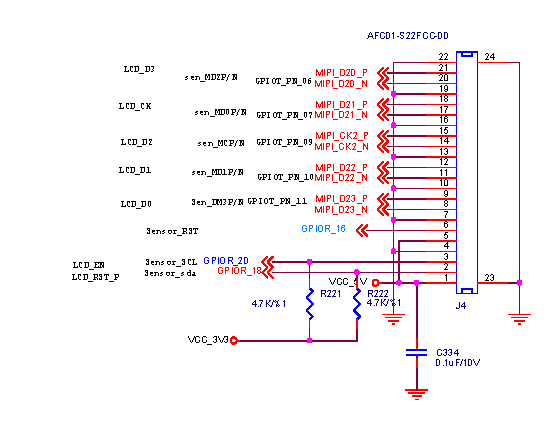
\includegraphics[width=.91\linewidth,height=2.7cm,keepaspectratio,trim={70bp 9bp 7bp 114bp},clip]{figures/camera_j4.pdf}\\[-1pt]
{\small (a) J4控制线与上拉电阻}
\end{minipage}\hfill
\begin{minipage}[b]{.46\linewidth}\centering
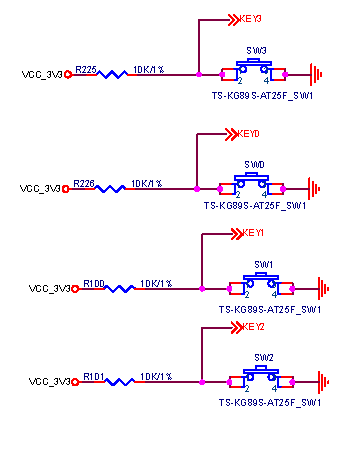
\includegraphics[width=.91\linewidth,height=2.7cm,keepaspectratio,trim={0bp 163bp 0bp 0bp},clip]{figures/keys_circuit.pdf}\\[-1pt]
{\small (b) KEY3按下接地}
\end{minipage}
\caption{摄像头控制与按键输入的局部电路，摘自Ti60 V4板级原理图\cite{board}。}\label{fig:hw-small}
\end{figure}
